%%%%%%%%%%%%%%%%%%%%%%%%%%%%%%%%%%%%%%%%%%%%%%
\section{Run Plan}
\label{sec:runplan}

To formulate a preliminary run plan, we assume the hadron beam spectrum and rates are as given in Tables~\ref{tab:beampartcomp} and~\ref{tab:beampartrates}.   For the purpose of estimating the beam time request, an average trigger/data rate of 50~Hz to tape is assumed.
\fixme{IMPORTANT: you should assume 25 Hz for any data run duration estimates and requests!  Otherwise we may find ourselves in a situation where we can only record ~50\% of our envisaged samples; on the other hand if we manage to run at 50Hz we'll always find other useful things to do ...}

For the run scenario in which we take 10k beam spills (two 4.8-s spills per SPS Super-cycle) for each momentum bin from 1 to 7~GeV/c at 1~GeV/c steps, the resulting sample for the positive beam is shown in Table~\ref{tab:RunPlan}. 

\begin{cdrtable}[Run Plan]{cccccccc}{RunPlan}{A preliminary run plan for ProtoDUNE-SP. The expected sample (positive beam) as a function of momentum is shown. }
P (GeV/c) & \# of spills &\# of $e^+$ & \# of $K^+$ & \# of $\mu^+$ & \# of $p$ & \# of $\pi^+$ & Total \# of Events \\ \toprowrule
1 & 10K & 672K & $\approx$ 0 & $\approx$ 0 & 192K & 144K & 1M \\ \colhline
2 & 10K & 480K & $\approx$ 0 & $\approx$ 0 & 336K & 480K & 1.3M \\ \colhline
3 & 10K & 1.5M & 17K  & 17K                & 203K  & 642K  & 2.4M \\ \colhline
4 & 10K & 1.1M & 49K & 33K                 & 197K & 1M & 2.4M \\ \colhline
5 & 10K & 896K  & 64K  & 16K               & 208K  & 1.2M & 2.4M \\ \colhline
6 & 10K & 667K & 99K  & 14K                & 241K  & 1.4M & 2.4M \\ \colhline
7 & 10K & 502K & 110K & 24K                & 257K  & 1.5M & 2.4M \\ \colhline
 & & & & & & & \\
Total & 70K & 5.9M & 340K & 104K & 1.6M & 6.4M & 14M \\
\end{cdrtable}

A similar table is also expected for the negative beam sample. \fixme{A table with similar values? Anne}

Preliminary beam simulations show that the hadron rates at 
energies below 1~GeV/c are low. Moreover, low-energy beams are more
subject to disruption and degradation by materials in the
beamline.  Therefore, the beam program factors in both the beam composition and %also takes into account of 
particle interaction topologies.  Full FLUKA\cite{fluka05,Fluka15}
 simulations
of particle transport in the the ProtoDUNE-SP detector, including the
beam window, have been performed.
 The physics requirement \fixme{that the beam must satisfy overall? Anne} is %the possibility 
 to enable measurement of
 stopping particles and  interactions at both high and low energies.    
%
At a beam momentum of 1~GeV/c, 35\% of protons stop, while the percentage reduces to only 5
per mill at 2~GeV/c. 
\fixme{use same units, \% or per mill (per thousand?)}  At  1~GeV/c,  the protons interact at all
energies as shown in
Figure~\ref{fig:pandpiint}. 
\fixme{protons of all energies interact? Anne}
The residual energy at the interaction
point can be reconstructed by measuring the energy deposited along the proton track.
Many of the  low-energy pions decay in the 37~m between the secondary target
and the LAr volume.  The fraction of stopping $\pi$'s for one $\pi$
leaving the target is 3\% at $p=0.4$~GeV/c,  %still  
1.3\% at $p=0.7$~GeV/c,
then decreases.  Having a $\pi$ beam at 0.7~GeV/c still allows 
measurement of pion interactions down to few tens of MeV with good
statistics. In a 1-GeV/c beam, the low-energy interactions are %still
present, albeit at a %with 
lower rate, as shown in Figure~\ref{fig:pandpiint}.
%
As for kaons, the length of the beamline is such that no
$K$ arrives at the detector for momenta lower than $\approx$2~GeV/c.
\fixme{``no $K$ with momentum lower than $\approx$2~GeV/c arrives at the detector'' Anne}
As for electrons, the peculiar topology of very low-energy electron-initiated 
showers requires a measurement at the lowest possible momenta.
\begin{cdrfigure}[Energy at interaction]{pandpiint}{Kinetic energy of
    particles at the point of interaction in the ProtoDUNE-SP active
    volume, for different beam momenta. Histograms are normalized to one particle injected in the
    beamline acceptance. FLUKA simulations include the beam window
    materials, beams are considered as monochromatic and
    parallel. Left: protons, Right: pions.}
  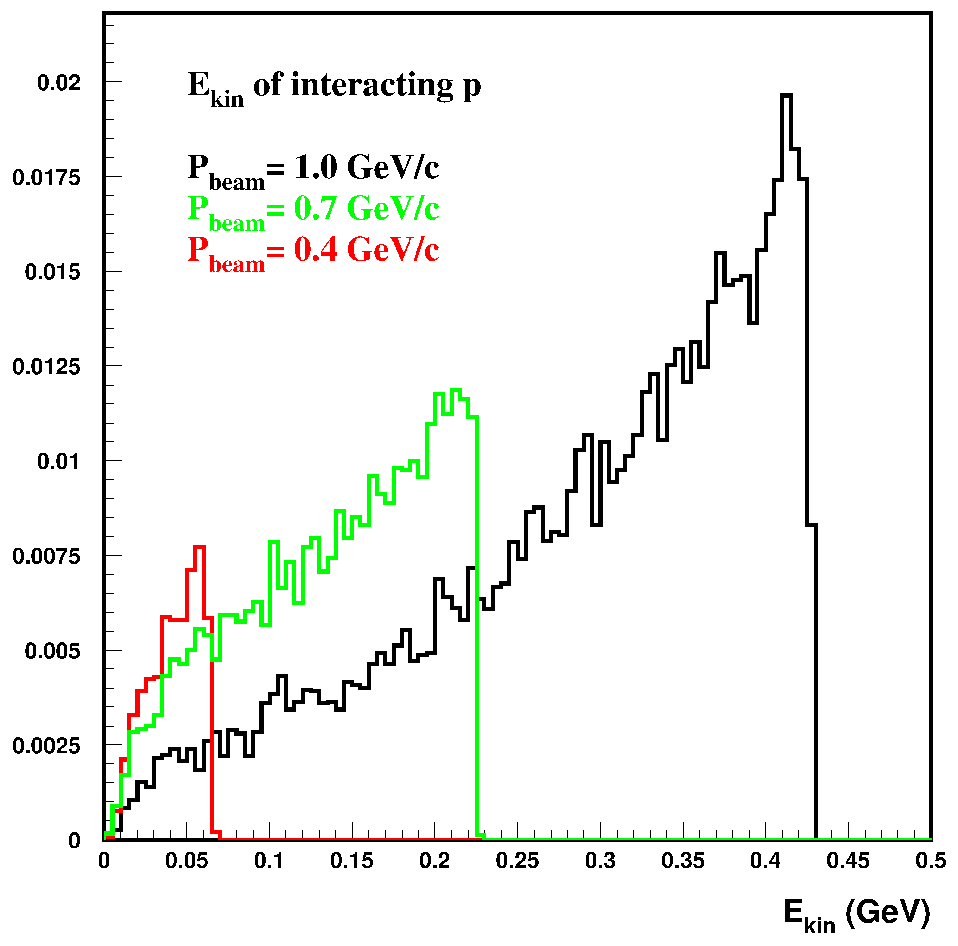
\includegraphics[width=0.49\textwidth]{pvarie_intene.pdf}
  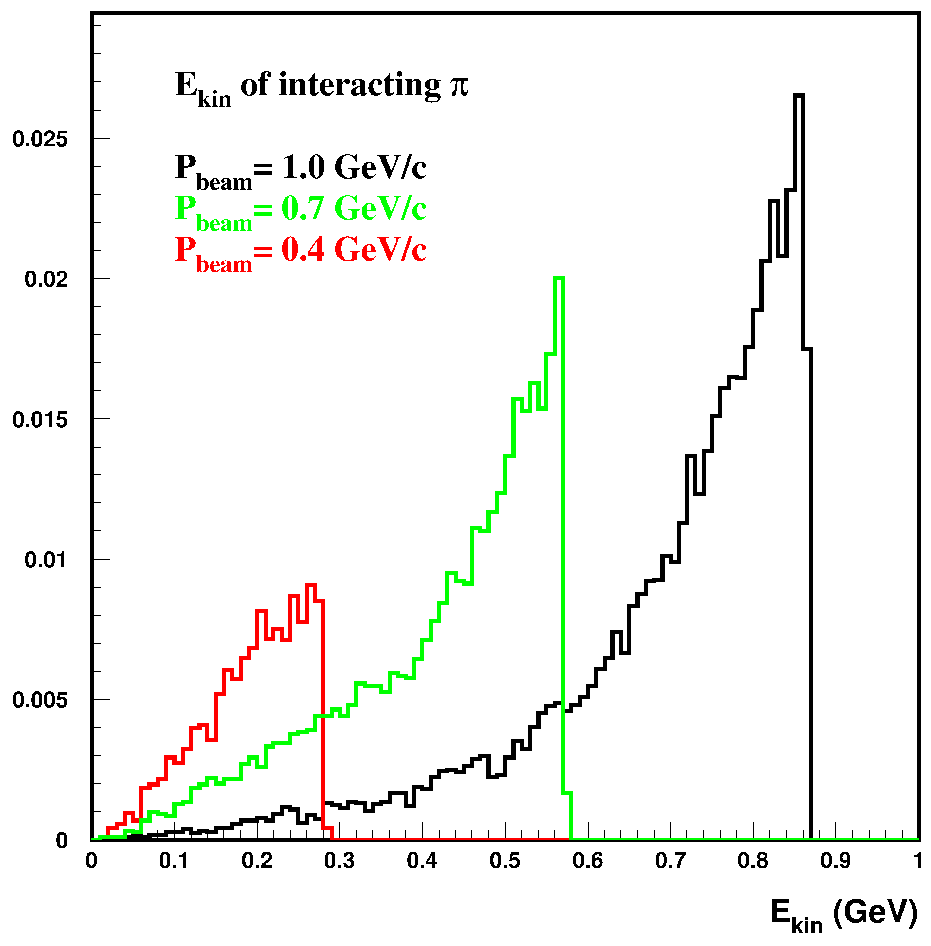
\includegraphics[width=0.49\textwidth]{pivarie_intene.pdf}
\end{cdrfigure}
%% end of   part that can go either here or in the run plan 

\fixme{Please make a separate table with estimates for $<$1 GeV hadrons and also electrons.}

In addition to the hadron beam run, there is an option to take some electron samples down to 0.5~GeV/c if requested by the physics group. 
\fixme{This has already been requested - please include it in your run plan.}
Based on the current information available, the total estimated beam time needed to carry out the physics program in this proposal is on the order of six weeks.
\fixme{never underestimate the beam time you need; err on the high side !}
 
 



